\chapter{\textbf{Introduction}}
\label{ch:intro}

Understanding the origin of the elements has been the primary goal of nuclear astrophysics since its conception. Through the work of Burbidge, Burbidge, Fowler, and Hoyle \cite{Burbidge1957}, it was established that the chemical elements observed in our solar system were synthesized through nuclear burning in stars. Indeed, all but the smallest elements in our observable universe (hydrogen through boron) are the ashes of stellar burning. Consequently, in the quest to discover the nature of the elemental origins, we must understand the nature of stellar processes. From birth to death, stars undergo nuclear reactions in their interiors. With sufficient temperatures, the reaction products themselves undergo subsequent nuclear reactions. An evolutionary stage is reached at which point the star either explodes or otherwise ejects its material outward. This nuclear-processed material is mixed together with the ashes from neighboring stars, forming new stars with new compositions and therefore new nucleosynthesis. One of the most complex evolutionary stages of a star is known as the asymptotic giant branch (AGB) phase, and stars that we currently observe on this phase are known as AGB stars. This thesis focuses on these complex nucleosynthesis processes in massive AGB stars, including s-process nucleosynthesis resulting from thermal pulses, as well as hot-bottom burning at the base of the convective hydrogen envelope. These stellar processes are investigated through laboratory nuclear reaction experiments here on earth. In particular, transfer reaction experiments are used in this thesis as a surrogate for the direct reactions occurring in the stellar processes. These experiments provide information on the nuclear structure of the nuclei involved in the key reactions, and therefore they constrain the reaction rates that are crucial to nucleosynthesis.

The present chapter will provide an overview of the nuclear astrophysics topics addressed in this thesis. Chapter \ref{ch:reactions} will introduce the mathematical formalism for quantifying nucleosynthesis with reaction rates, as well as the formalism for transfer reactions. Chapter \ref{ch:Rb} will address the ``rubidium problem'' in massive AGB stars, a descrepancy between observed and theoretical rubidium abundances from s-process nucleosynthesis. The s-process branching at $^{86}$Rb is investigated through a Monte Carlo reaction network approach, identifying the most important reactions to rubidium abundance.
%The measurements of the $^{86}\mathrm{Kr}(^{3}\mathrm{He},d)^{87}\mathrm{Rb}$ transfer reaction and the $^{87}\mathrm{Rb}(\gamma,\gamma')^{87}\mathrm{Rb}$ and $^{87}\mathrm{Rb}(\gamma,n)^{86}\mathrm{Rb}$ photoabsorption reactions are proposed to enhance our understanding of the closed-N shell nucleus $^{87}$Rb and its involvement in the rubidium overabundance. 
Chapter \ref{ch:exp} will introduce the experimental techniques that were used in this thesis to successfully perform transfer reaction experiments. Chapter \ref{ch:DAQ} will introduce the development of a new digital data acquisition system (DAQ) for the focal-plane detector package at the Enge Split-Pole Spectrograph, which will replace the current analog system for future transfer reaction experiments. Finally, Chapter \ref{ch:GC} will address the Mg--K abundance anomaly observed in globular cluster NGC 2419, which may have originated from hot-bottom burning in massive AGB stars. The $^{39}\mathrm{K}(^{3}\mathrm{He},d)^{40}\mathrm{Ca}$ proton-transfer reaction is measured at high resolution, and new constraints are placed on the key potassium-destroying reaction $^{39}\mathrm{K}(p,\gamma)^{40}\mathrm{Ca}$.

% PUT THIS IN THE ABSTRACT:
%Four resonances in $^{39}\mathrm{K}+p$ are resolved for the first time.
%from the first-ever resolution of the 154 keV resonance in $^{39}\mathrm{K}+p$.
% Nuclear reaction network calculations will show the how the new reaction rate

%--------------------------------------------------------------------------
%--------------------------------------------------------------------------
\section{Asymptotic Giant Branch Stars}
% Evolution on the H-R diagram (figure). Early (E-AGB) phase versus thermally-pulsing (TP-AGB) phase. The hydrogen and helium burning shells in the TP-AGB phase (with figure). S-Process occuring in the inter-shell region during and between thermal pulses. Hot-bottom burning occuring between the base of the convective hydrogen envelope and the hydrogen-burning shell.

Asymptotic giant branch (AGB) stars produce about half of all elements heavier than iron in our galaxy \cite{Busso1999}, and they are one of the leading candidates for the origin of abundance anomalies in globular clusters \cite{Prantzos2007}. An understanding of these stars therefore provides insight into the origin of the elements. The asymptotic giant branch refers to the evolutionary track that these stars follow on a typical Hertzsprung-Russell (HR) diagram, which asymptotically approaches that of the red giant branch. HR diagrams show the luminosity of a star as a function of its effective temperature. These properties are often cataloged for each star observed in a globular cluster, for example, and the current evolutionary phase of a star can be determined from its relative position on the diagram. A theoretical example of the evolutionary track of a 5 $M_{\odot}$ star is represented on the HR diagram of Fig. \ref{fig:5M_Evolution}. Starting from the zero-age main sequence (ZAMS), where the star first begins to burn hydrogen, the evolutionary track passes through the sub-giant branch (SGB), the red-giant branch (RGB), the horizontal branch (HB), the early (E-) and thermally-pulsing (TP-) asymptotic giant branch (AGB) phases, and the post-AGB branch. It then undergoes planetary nebula (PN) formation, before eventually becoming a white dwarf. Each of these branches represents a unique evolutionary phase of the star, many of which are described in the figure at key transitional points. As mentioned above, this thesis focuses on AGB stars, the evolutionary track of which is highlighted in red in the figure.

\begin{figure}[t]
\centering
\begin{tikzpicture}[scale=1.0, every node/.style={transform shape}]
\coordinate (a) at (3,1.7);
\coordinate (b) at (4.14,3.52);
\node at (0,0) {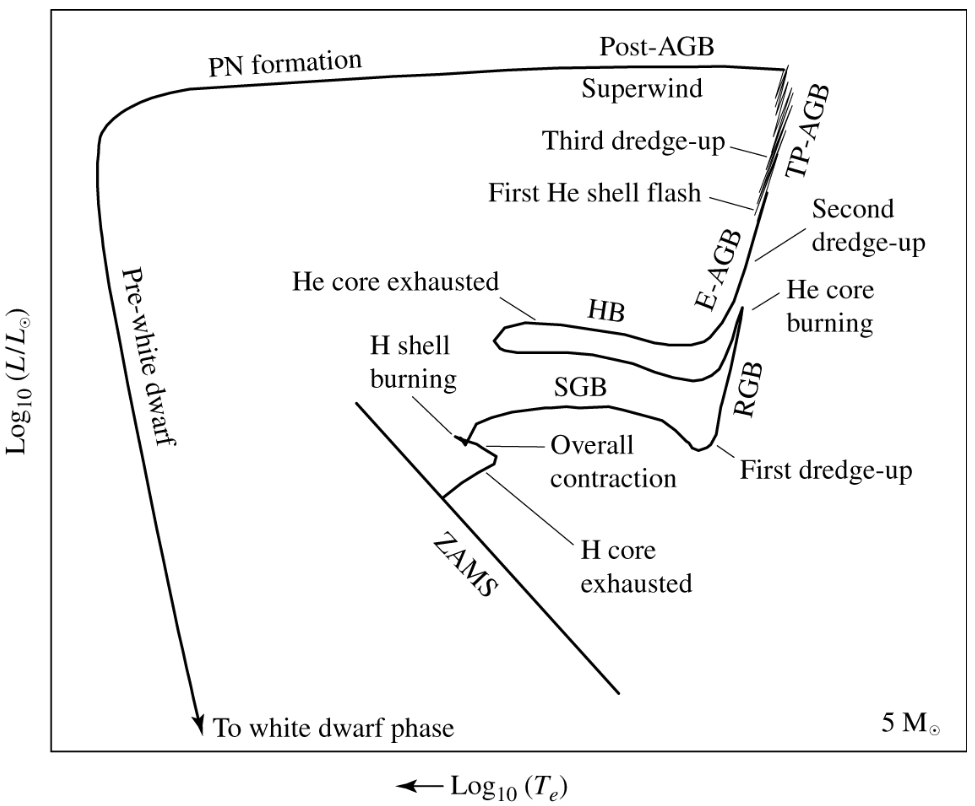
\includegraphics[width=5in]{Chapter-1/figs/5M_Evolution.png}};
\draw[rotate around={72:(a)},color=red] (a) ellipse (0.8 cm and 0.3 cm);
\draw[rotate around={72:(b)},color=red] (b) ellipse (0.8 cm and 0.3 cm);
\end{tikzpicture}
\caption{\label{fig:5M_Evolution}Evolution of a 5 $M_{\odot}$ star represented on the Hertzsprung-Russell (HR) diagram. The two stages of the asymptotic giant branch (AGB) are highlighted in red. See text for definitions of acronyms. Figure adapted from Ref. \cite{Carroll2007}.}
\end{figure}

It is clear from Figure \ref{fig:5M_Evolution} that AGB stellar evolution is separated into two stages. The \emph{early-AGB} (e-AGB) stage occurs after both hydrogen and helium have been exhausted in the core of a star, leaving behind mostly inert carbon and oxygen. Hydrogen and helium burning is still active in separate shells around the core, with a helium-rich intershell region in between. The far more active hydrogen-burning shell perpetually increases the density and temperature of the intershell region, until the rate of energy generated by the helium-burning shell is greater than the rate at which energy can be transported outward through radiative diffusion \cite{Iliadis2015}. A thermal instability, called a \emph{thermal pulse}, occurs as a result, initiating the \emph{thermally pulsing AGB} (TP-AGB) stage, shown in Figure \ref{fig:AGB_Structure}. This pulse causes the helium-burning shell to extend into the intershell region and ignite the hydrogen-burning shell, rendering it inactive for a brief period. The nuclei inside the intershell region get carried outward through the convective hydrogen envelope toward the surface of the star, in what is known as a \emph{third dredge-up} (3DUP) event\footnote{The first two dredge-ups are depicted in Figure \ref{fig:5M_Evolution}, occurring at the start of the RGB and during the e-AGB stage, respectively. For stars with $M \lesssim 4 \, M_{\odot}$, the second dredge-up does not occur because the convective hydrogen envelope cannot penetrate the intershell region at this point.}, where they are ejected by stellar winds. The hydrogen-burning shell takes over once again as the dominant energy-producer after the thermal pulse, and this cycle repeats for on the order of tens to hundreds of pulses \cite{Habing2004}.

%\begin{figure}[t]
%\centering
%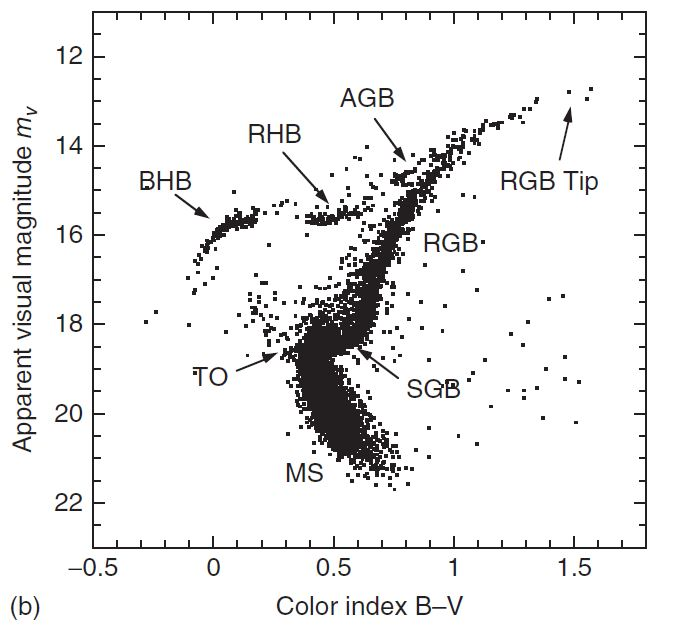
\includegraphics[width=5in]{Chapter-1/figs/HRDiagram.jpg}
%\caption{\label{fig:HRDiagram}The Hertzsprung-Russell (HR) diagram. Figure adapted from Ref. \cite{Iliadis2015}.}
%\end{figure}

\begin{figure}[t]
\centering
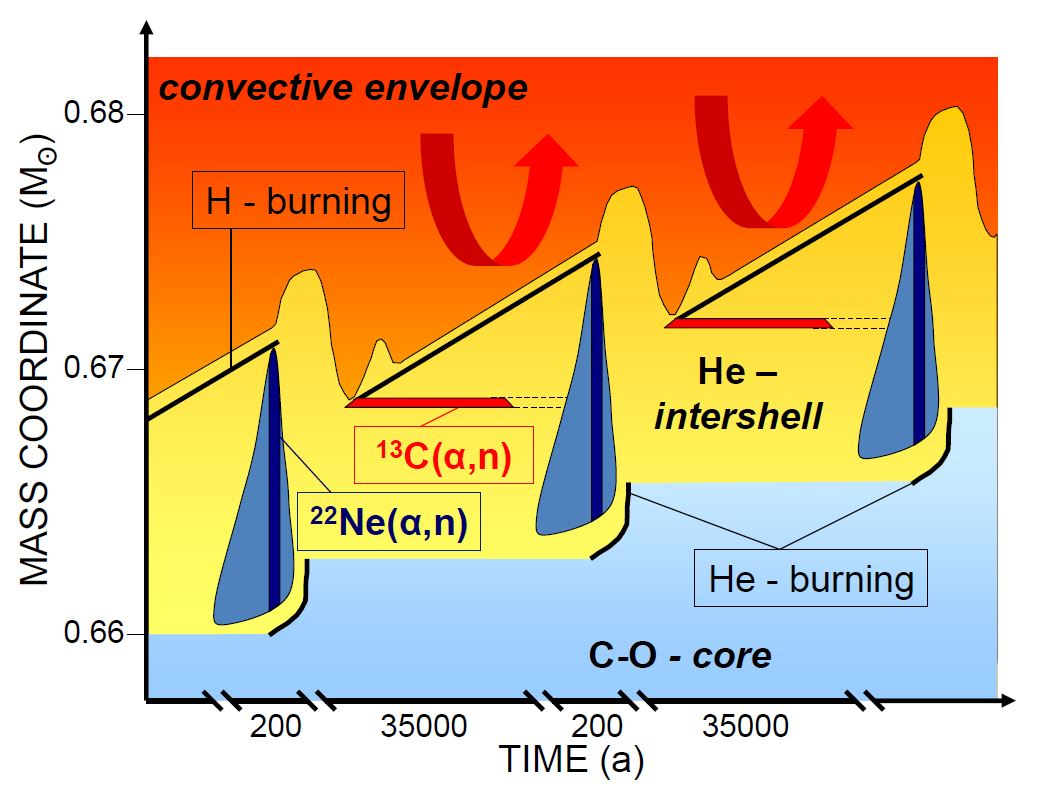
\includegraphics[width=6.5in]{Chapter-1/figs/sProcess_AGB.JPG}
\caption{\label{fig:AGB_Structure}The evolution and structure of a thermally pulsing AGB star. Three thermal pulses are depicted in blue, extinguishing the hydrogen burning shell. The neutron sources $^{13}\mathrm{C}(\alpha,n)^{16}\mathrm{O}$ and $^{22}\mathrm{Ne}(\alpha,n)^{25}\mathrm{Mg}$ are shown to be active between pulses and during pulses, respectively. Figure adapted from Ref. \cite{Reifarth2014}.}
\end{figure}

Helium burning during each thermal pulse produces $^{12}$C as a result of the triple-$\alpha$ reaction, followed by $^{16}$O from $^{12}\mathrm{C}(\alpha,\gamma)^{16}\mathrm{O}$, which get accumulated mostly in the core, increasing its mass. However, some $^{12}$C accumulates in the intershell region. After a 3DUP event resulting from a thermal pulse, some protons from the convective hydrogen envelope mix into the intershell region, initiating the reaction sequence $^{12}\mathrm{C}(p,\gamma)^{13}\mathrm{N}(\beta^{+}\nu)^{13}\mathrm{C}(p,\gamma)^{14}N$. The effect of these additional proton-capture reactions is the formation of a \emph{$^{13}$C pocket} and a \emph{$^{14}$N pocket} at the top of the intershell region. During the interpulse period, when temperatures are between $100$ MK $\lesssim T \lesssim$ 300 MK, the $^{13}\mathrm{C}(\alpha,n)^{16}\mathrm{O}$ reaction is activated, producing a large neutron density of $N_{n} \approx 10^{7}$ $\mathrm{cm}^{-3}$. During thermal pulses, when temperatures are $T \gtrsim 300$ MK, the reaction sequence $^{14}\mathrm{N}(\alpha,\gamma)^{18}\mathrm{F}(\beta^{+}\nu)^{18}\mathrm{O}(\alpha,\gamma)^{22}\mathrm{Ne}$ proceeds. As a result, the $^{22}\mathrm{Ne}(\alpha,n)^{25}\mathrm{Mg}$ reaction is activated, producing an even larger neutron density of $N_{n} \approx 10^{10}$ $\mathrm{cm}^{-3}$. Nucleosynthesis occurs in the intershell region from these two neutron sources via a series of neutron-captures and $\beta$--decays, known as the s-process, described in Section \ref{sec:s-process}. The heavy nuclei produced from the s-process are brought to the surface by subsequent thermal pulses and 3DUP events.
%The overabundance of rubidium as a result of the s-process in massive AGB stars is described in Section \ref{subsec:Rb_Overabundance}.

In the case of AGB stars with $M \gtrsim 4 \, M_{\odot}$, the convective hydrogen envelope reaches down to the top of the hydrogen-burning shell during the interpulse period, where temperatures are $T \gtrsim 50$ MK \cite{Iliadis2015}, but can theoretically reach as high as $T \approx 150$ MK for \emph{Super-AGB} (SAGB) stars with $M \gtrsim 7 \, M_{\odot}$ \cite{Ventura2012}. The resulting hydrogen burning nucleosynthesis is known as hot-bottom burning, detailed in Section \ref{sec:hot-bottom-burning}, and the products of this burning are brought to the surface by the convective hydrogen envelope. This process is one of the leading candidates for the recent abundance anticorrelations observed in globular clusters, detailed in Section \ref{subsec:GC_Candidate}.

%--------------------------------------------------------------------------
%--------------------------------------------------------------------------
\section{s-Process Nucleosynthesis} \label{sec:s-process}
% Main and weak components of the s-process here
% s-process paths picture

% Both during thermal pulses and during the interpulse period, the helium-rich intershell region produces a large flux of neutrons. These neutrons originate from the neutron sources, $^{13}\mathrm{C}(\alpha,n)^{16}\mathrm{O}$ and $^{22}\mathrm{Ne}(\alpha,n)^{25}\mathrm{Mg}$. The former reaction is the dominant neutron source during the interpulse period, where temperatures are between about $100$ MK $\lesssim T \lesssim$ 300 MK and neutron densities are roughly $N_{n} \approx 10^{7}$ $\mathrm{cm}^{-3}$. During thermal pulses, where $T$ and $N_{n}$ increase, the latter reaction is dominant and occurs at $T \gtrsim 300$ MK and $N_{n} \approx 10^{10}$ $\mathrm{cm}^{-3}$. Nucleosynthesis occurs in the intershell region via a series of neutron captures and beta decays, known as the s-process, described in Section \ref{sec:s-process}.

% Neutrons lead to nucleosynthesis for A>60

Most light nuclei below the iron-peak at mass number $A \approx 60$ are formed through charged-particle fusion reactions in stars, where temperatures are sufficient for transmission through the repulsive Coulomb barrier via quantum tunneling. The synthesis of nuclei heavier than the iron-peak, however, cannot be explained by these charged-particle fusion reactions. At low temperatures, the transmission probability through the large Coulomb barrier of heavy nuclei becomes prohibitively small, while at high temperatures, nuclear statistical equilibrium favors the production of iron-peak nuclei due to their large binding energy per nucleon. Nuclei with $A \gtrsim 60$ must be formed instead by neutron capture, where Coulomb repulsion is no longer a factor. Neutron capture will generate neutron-rich isotopes of a given element, some of which eventually undergo $\beta$--decay if they are unstable. The stable daughter nuclei will then capture neutrons until another unstable isotope is reached, and the process continues this way up to some of the heaviest nuclei.

%--------------------------------------------------------------------------
% s-process vs r-process

When the neutron density in the astrophysical environment is sufficiently small such that unstable nuclei preferentially $\beta$--decay, the ensuing nucleosynthesis is referred to as the \emph{s-process}. This is a relatively slow process (hence the \emph{s-}), as the nucleosynthesis can only proceed based on the half-lives of the unstable nuclei. If, on the other hand, the neutron density is sufficiently large such that unstable nuclei preferentially neutron-capture, the ensuing nucleosynthesis is referred to as the \emph{r-process} because this happens at a much more (\emph{r-})apid pace. These two processes occur in different astrophysical sites and are equally responsible for almost all of the heavy nuclei in the observable universe. Some heavy nuclei are referred to as s-only or r-only nuclei because only one of these processes accounts for their abundance. The research presented in Chapter \ref{ch:Rb} is based on s-process nucleosynthesis occurring in AGB stars.

%--------------------------------------------------------------------------
% s-process path and abundance evolution

\begin{figure}[t]
\centering
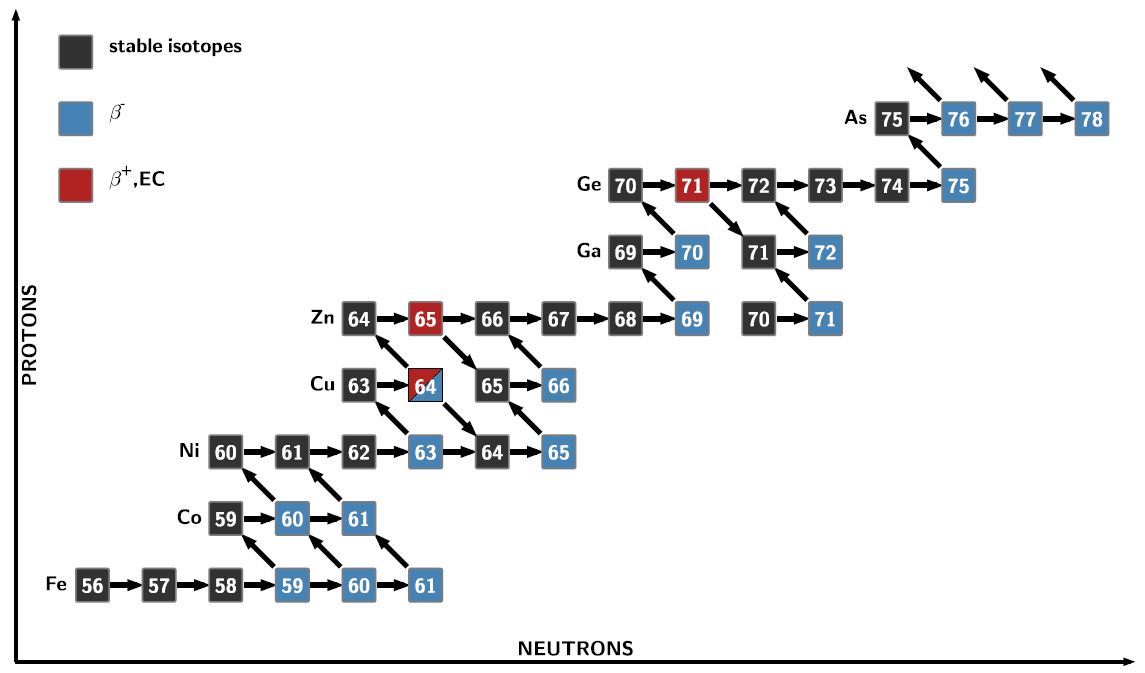
\includegraphics[width=6.5in]{Chapter-1/figs/sProcess_path.jpg}
\caption{\label{fig:sProcess_path}The s-process path from iron to arsenic. The stable nuclei in black undergo neutron capture, while the unstable nuclei in blue ($\beta^{-}$-decay) and red ($\beta^{+}$-decay or electron capture) either decay or undergo neutron-capture depending on their half-lives and the neutron density $N_{n}$. At s-process branchings, e.g. $^{59}$Fe, the probability for neutron-capture and decaying is approximately equal, hence the path is split into two branches. Figure adapted from Ref. \cite{Reifarth2014}.}
\end{figure}

To illustrate how the s-process works, consider the chain of reactions shown in Figure \ref{fig:sProcess_path}, starting with the most abundant stable nucleus formed at the end of the stellar fusion reaction chains, $^{56}$Fe. This is referred to as a \emph{seed nucleus} because it is the nucleus that initiates the s-process reaction chain. Stable nuclei are shown in black in the figure, nuclei unstable to $\beta^{-}$--decay are shown in blue, and nuclei unstable to $\beta^{+}$--decay or electron capture (EC) are shown in red. As is typical of a chart of the nuclides, neutron number increases to the right and proton number increases upward. Neutron-capture is therefore represented by an arrow to the right, while $\beta$--decays and electron capture are represented by diagonal arrows due to the conversion of a neutron to a proton, or vice versa. If there is a sufficient neutron density $N_{n}$ in the astrophysical environment, the neutron-capture of $^{56}$Fe, $^{56}\mathrm{Fe}(n,\gamma)^{57}\mathrm{Fe}$, leads to the stable nucleus $^{57}$Fe. The two subsequent neutron-captures,  $^{57}\mathrm{Fe}(n,\gamma)^{58}\mathrm{Fe}$ and  $^{58}\mathrm{Fe}(n,\gamma)^{59}\mathrm{Fe}$, on the stable $^{57}$Fe and $^{58}$Fe nuclei, respectively, leads to the unstable $^{59}$Fe nucleus. The nucleosynthesis path has now lead to an \emph{s-process branching}, and $^{59}$Fe is referred to as a \emph{branching point nucleus}. At these branchings, the decay constant for $\beta$--decay, $\lambda_{\beta}$, is approximately equal to the decay constant for neutron capture, $\lambda_{n\gamma}$. That is, $\lambda_{\beta} \approx \lambda_{n\gamma}$, and the path splits into two branches with approximately equal probability. These branchings are sensitive to neutron density $N_{n}$ and the neutron-capture cross section $\sigma_{n\gamma}$ of the unstable branching point nucleus, described below. After the s-process branching, the path continues in this way up to some of the heaviest nuclei.

% "Classical" s-process (Eqns. 5.173 - 5.192 in Nuclear Physics of Stars). Disregards time dependence of s-process parameters, such as neutron density and stellar temperature. Makes no assumption on the stellar site or specific reactions acting as neutron sources. The classical model offers remarkable insight into the s-process regardless. It explains the main, weak, and strong s-process components. Eqn. 5.192 describes the simplest case of an s-process branching, but each branching is different. 

% Include custom simple neutron capture and beta decay figure with a branching.
% Include figure of overall Reifarth s-process path.
% For math, maybe only include 2 sets of equations - 5.173 to 5.174 and 5.191 (excluding the tau part) to 5.192 (excluding the top line) --- Don't need Tau for any of these!

% Use Nuclear Physics of Stars Figure 5.68 parts (b) and (c) with the math. Part (b) assumes radioactive nuclei always undergo beta-decay. Can start from Eqn. 5.173, even removing part (a).

\def\BoxSpace{0.3} % Defining the variable BoxSpace to value in brackets
\def\BoxSpacetwo{\BoxSpace * 2} % So I don't have to keep doing {2+(\BoxSpace * 2)}
\def\BoxSpacethree{\BoxSpace * 3}
\def\BoxSpacehalf{\BoxSpace * 0.5}
\def\AOS{0.15} % Arrow Offset
\def\AW{0.52} % Arrow Width (mm)

\begin{figure}[t]
\centering
\begin{tikzpicture}[scale=2.0, every node/.style={transform shape}]

\filldraw[fill = light-gray] (0,0) rectangle (1,1); % A-1
\filldraw[fill = light-gray] (0,1+\BoxSpace) rectangle (1,2+\BoxSpace); % A
\filldraw[fill = light-gray] (1+\BoxSpace,1+\BoxSpace) rectangle (2+\BoxSpace,2+\BoxSpace); % A+1
\draw (1+\BoxSpace,0) rectangle (2+\BoxSpace,1); % A'
\filldraw[fill = light-gray] (2+\BoxSpacetwo,1+\BoxSpace) rectangle (3+\BoxSpacetwo,2+\BoxSpace);% A+2
\draw (2+\BoxSpacetwo,0) rectangle (3+\BoxSpacetwo,1); % A'+1

\node at (0.5,0.5) {\scriptsize{$A\!-\!1$}};
\node at (0.5,1+\BoxSpace+0.5) {\scriptsize{$A$}};
\node at (1+\BoxSpace+0.5,1+\BoxSpace+0.5) {\scriptsize{$A\!+\!1$}};
\node at (1+\BoxSpace+0.5,0.5) {\scriptsize{$A'$}};
\node at (2+\BoxSpacetwo+0.5,1+\BoxSpace+0.5) {\scriptsize{$A\!+\!2$}};
\node at (2+\BoxSpacetwo+0.5,0.5) {\scriptsize{$A'\!+\!1$}};

\draw[line width = \AW mm, -{Triangle[]}] (1-\AOS,0.5) -- (1+\BoxSpace+\AOS,0.5); % A-1(n,g)
\draw[line width = \AW mm, -{Triangle[]}] (1+\BoxSpace+\AOS,1-\AOS) -- (1-\AOS,1+\BoxSpace+\AOS); % A' beta-decay
\draw[line width = \AW mm, -{Triangle[]}] (1-\AOS,1+\BoxSpace+0.5) -- (1+\BoxSpace+\AOS,1+\BoxSpace+0.5); % A(n,g)
\draw[line width = \AW mm, -{Triangle[]},dashed] (2+\BoxSpace-\AOS,1+\BoxSpace+0.5) -- (2+\BoxSpacetwo+\AOS,1+\BoxSpace+0.5); %A+1(n,g)
\draw[line width = \AW mm, -{Triangle[]},dashed] (2+\BoxSpace-\AOS,0.5) -- (2+\BoxSpacetwo+\AOS, 0.5); %A'(n,g)
\draw[line width = \AW mm, -{Triangle[]},dashed] (2+\BoxSpacetwo+\AOS,1-\AOS) -- (2+\BoxSpace-\AOS,1+\BoxSpace+\AOS); %A'+1 beta-decay

\end{tikzpicture}
\vspace{0.75 cm}
\caption{\label{fig:sProcess_MathExample}A simple s-process path initiating from the nucleus with mass number $A-1$, where shaded nuclei are stable and unshaded nuclei are unstable. The simplest case, where only $\beta$--decays occur on unstable nuclei, is shown by the solid arrows. The added complication of a branching at $A'$ is indicated by dashed arrows.}
\end{figure}

Now consider the simple s-process path shown in Figure \ref{fig:sProcess_MathExample}, starting from a stable nucleus with mass number $A-1$. In the simplest case represented by solid arrows, the unstable nucleus with mass number $A'$ will $\beta$--decay to nucleus $A$, which will then neutron-capture to nucleus $A+1$, and so on. The more complicated case is represented by dashed arrows, where the nucleus $A'$ is at a branching, and it can undergo neutron-capture and $\beta$--decay at roughly equal probability. We will first assume that $\lambda_{\beta} >> \lambda_{n\gamma}$, such that the path does not lead through the dashed arrows. In this case, the abundance at each mass number exists in only one (unprimed) nucleus. Therefore the abundance evolution of any stable nucleus $A$ only depends on the neutron-capture reaction rates of the $A-1$ and $A$ nuclei, as in
\begin{equation} \label{eqn:sProcess_AbundEvol}
\frac{dN_{s}(A)}{dt} = N_{n}(t)N_{s}(A-1)\langle \sigma v \rangle_{A-1} - N_{n}(t)N_{s}(A)\langle \sigma v \rangle_{A},
\end{equation}
where $N_{s}(A)$ and $N_{n}(t)$ are the time-dependent number densities of the $A$ nucleus and the neutron, respectively, and $\langle \sigma v \rangle_{A}$ is the neutron-capture reaction rate per particle pair of the $A$ nucleus. The first term in Eqn \ref{eqn:sProcess_AbundEvol} represents the rate of production of the $A$ nucleus, while the second term represents its rate of destruction. We will assume that the temperature is constant while the neutron source is active, so that the neutron-capture reaction rates are also constant. The neutron-capture reaction rate is frequently expressed in terms of a Maxwellian-averaged cross section $\langle \sigma \rangle_{A} \equiv \langle \sigma v \rangle_{A} / v_{T}$, where $v_{T} = \sqrt{2kT/\mu_{An}}$ is the thermal velocity, or in other words, the maximum of the velocity distribution; $\mu_{An}$ is the reduced mass between the $A$ nucleus and the neutron, which is approximately equal to the neutron mass. That is, $\mu_{An} = M_{A}M_{n}/(M_{A} + M_{n}) \approx M_{n}$, which makes $v_{T}$ approximately independent of target mass. The abundance evolution of the nucleus $A$ can then be written as
\begin{equation}
\frac{dN_{s}(A)}{dt} = v_{T}N_{n}(t) \, \left[ N_{s}(A-1)\langle \sigma \rangle_{A-1} - N_{s}(A)\langle \sigma \rangle_{A} \right].
\end{equation}

Far from any s-process branchings or closed neutron-shell nuclei, an approximate equilibrium is obtained where the abundance of the $A$ nucleus increases until its production rate and destruction rate are approximately equal. This is known as the \emph{local equilibrium approximation}, and it is expressed as $N_{s}(A,\tau)\langle \sigma \rangle_{A} \approx N_{s}(A-1,\tau)\langle \sigma \rangle_{A-1}$, where $\tau$ is the neutron exposure, in units of neutrons per area. The neutron exposure is proportial to the time-integrated neutron flux $\Phi$, as in $\tau = (\sqrt{\pi}/2) \Phi$. The local equilibrium approximation has been shown to hold for the s-only isotopes of tellurium ($Z=52$), as well as for many other s-only nuclei with adjacent mass numbers between $90 \lesssim A \lesssim 205$ \cite{Iliadis2015}. However, there is a distinct separation of observed solar system $N_{\odot}(A)\langle \sigma \rangle_{A}$ values at $A \approx 90$, and the approximation does not hold at all near the closed neutron-shell nuclei. Refs. \cite{Clayton1961,Seeger1965} have shown that better agreement with solar system $N_{\odot}(A)\langle \sigma \rangle_{A}$ values is achieved when considering not just a single neutron exposure $\tau$, but an exponential distribution of $\tau$-values. Indeed, it is reasonable to assume that the number of $^{56}$Fe seed nuclei decreases with increased exposure to neutrons. With this additional constraint, the solar system $N_{\odot}(A)\langle \sigma \rangle_{A}$ values are reproduced to a remarkable accuracy for $90 \lesssim A \lesssim 205$, when also accounting for s-process branchings, discussed below. The region between $60 \lesssim A \lesssim 90$ is also reproduced with an exponential distribution of neutron exposures, but different parameters are required between the two cases. These two components are referred to as the \emph{main s-process component} ($90 \lesssim A \lesssim 205$) and the \emph{weak s-process component} ($60 \lesssim A \lesssim 90$). A third component, called the \emph{strong s-process component} is needed to explain the solar system $N_{\odot}(A)\langle \sigma \rangle_{A}$ values at $A \gtrsim 205$. 

%--------------------------------------------------------------------------
% weak-component vs main-component (vs strong-component?) in the s-process 

% Different sites (AGB, massive star), weak is for 60 < A < 90, main is 90 < A < 205, strong A > 205
% Treated separately, they describe all s-only nuclide abundances

These components originate from different astrophysical environments, where the total number of $^{56}$Fe seed nuclei and the exponential neutron exposure differ. The main s-process component is from thermally-pulsing AGB stars with $1.5 M_{\odot} \lesssim M \lesssim 3 M_{\odot}$, while the weak s-process component is thought to originate from core helium burning and shell carbon burning in massive stars with $M \gtrsim 13 M_{\odot}$ \cite{Iliadis2015}. The primary neutron source for the main component is $^{13}\mathrm{C}(\alpha,n)^{16}\mathrm{O}$, with the $^{22}\mathrm{Ne}(\alpha,n)^{25}\mathrm{Mg}$ neutron source only marginally activated. This latter source acts to enhance the efficiency of s-process branchings. The weak s-process component, however, relies on $^{22}\mathrm{Ne}(\alpha,n)^{25}\mathrm{Mg}$ as its primary neutron source, since temperatures are significantly higher for these massive stars.

If we now consider the nucleus $A'$ in Figure \ref{fig:sProcess_MathExample} as an s-process branching, we can see that only a fraction of the path reaches the nucleus $A$, but the entire path reaches the nucleus $A+1$. In this case, the local equilibrium approximation becomes $N_{s}(A,\tau)\langle \sigma \rangle_{A} + N_{s}(A',\tau)\langle \sigma \rangle_{A'} \approx N_{s}(A+1,\tau)\langle \sigma \rangle_{A+1}$. We can now define the \emph{branching ratio} $B$ as
\begin{align}
B &\equiv \frac{N_{s}(A,\tau)\langle \sigma \rangle_{A}}{N_{s}(A+1,\tau)\langle \sigma \rangle_{A+1}} = \frac{\lambda_{\beta}(A')}{\lambda_{\beta}(A') + \lambda_{n\gamma}(A')} \nonumber \\
&= \frac{\ln 2 / T_{1/2}(A')}{\ln 2 / T_{1/2}(A') + N_{n} \langle \sigma \rangle_{A'} v_{T}}.
\end{align}
Solving for the neutron number density $N_{n}$, we obtain
\begin{equation} \label{eqn:neutron_density}
N_{n} = \left( \frac{1-B}{B} \right) \frac{1}{\langle \sigma \rangle_{A'} v_{T}} \frac{\ln 2}{T_{1/2}(A')}.
\end{equation}
Even though Eqn. \ref{eqn:neutron_density} is just one of many examples of possible s-process branching configurations, it shows the only inputs necessary to calculate the neutron density, which is a key parameter in stellar models of the s-process. From this equation, a connection is made between the study of s-process branchings and the neutron density. 

In order to extract the neutron density with a reasonable uncertainty, it is crucial to have precise experimental neutron-capture cross sections of the $A$, $A+1$, and $A'$ nuclei. Since the $A$ and $A+1$ nuclei are stable, these are usually readily available. However, $A'$ is unstable, and it is typically not feasible to perform neutron-capture cross section measurements on unstable nuclei. In cases where data is not available, the cross sections have to be estimated using Hauser-Feshbach theory. It is possible to experimentally constrain neutron-capture cross sections on unstable nuclei by performing photoabsorption reactions on the recoil nucleus, if it is stable. The dipole response of the recoil nucleus via nuclear resonance fluorescence (NRF) and the $(\gamma,n)$ reaction can be used to determine the photoabsorption cross section of the recoil nucleus, which can in turn be used to determine its photon strength function (PSF). The PSF is a crucial input for statistical model calculations constraining Maxwellian-averaged cross sections of neutron-capture on unstable nuclei \cite{Wilhelmy2020}.

%--------------------------------------------------------------------------
%--------------------------------------------------------------------------
%\subsection{Rubidium Overabundance} \label{subsec:Rb_Overabundance}

% Not covering this because I'm also not covering Mg-K anticorrelation yet. Only introducing the main concepts - s-process and hot-bottom burning + globular cluster anticorrelations

\begin{figure}[t]
\centering
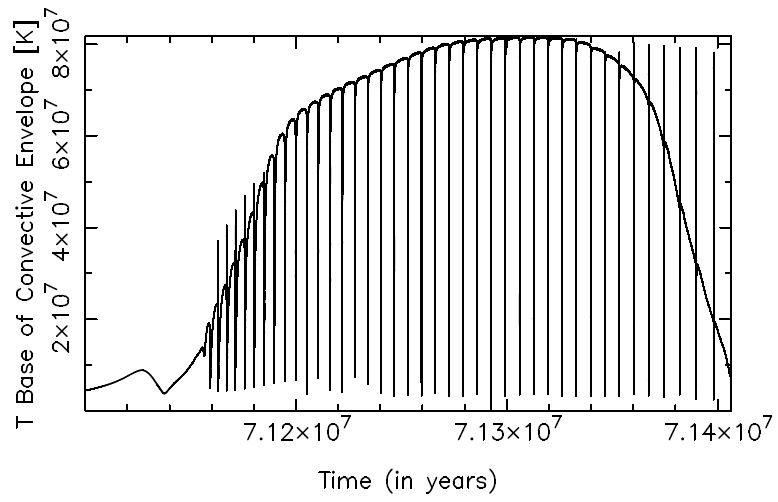
\includegraphics[width=6.5in]{Chapter-1/figs/HBB.jpg}
\caption{\label{fig:HBB}The temperature evolution at the bottom of the convective hydrogen evelope during the TP-AGB phase for a $6 M_{\odot}$ star with $Z=0.02$. Several thermal pulses are shown, each rapidly decreasing the temperature in this region, which extinguishes hydrogen burning. Adapted from Ref. \cite{Karakas2014}.}
\end{figure}

%--------------------------------------------------------------------------
%--------------------------------------------------------------------------
\section{Hot-Bottom Burning} \label{sec:hot-bottom-burning}

%In the case of massive AGB stars ($M \gtrsim 4 M_{\odot}$), the convective hydrogen envelope reaches down to the top of the hydrogen-burning shell during the interpulse period, where temperatures are at least 50 MK. The resulting hydrogen burning nucleosynthesis is called \emph{hot-bottom burning}

Hot-bottom burning (HBB) occurs in AGB stars when the bottom of the convective hydrogen envelope reaches sufficiently high temperatures for nuclear processing. The onset of HBB is highly dependent upon the AGB mass and metallicity, with a minimum mass of $\sim 5 M_{\odot}$ at solar metallicty $Z_{\odot}$, to even theoretically as low as $\sim 2 M_{\odot}$ at $Z=0$ \cite{Habing2004}. Temperatures can exceed 50 MK during HBB, which is sufficient to activate the CNO cycle, as well as the Ne-Na chain. For super-AGB stars and the most massive and lowest-metallicity AGB stars, temperatures can exceed 100 MK, which is sufficient to activate the Mg-Al and Ar-K chains \cite{Karakas2014}. HBB is only active during the interpulse period because thermal pulses act to cool down this region by about an order of magntidue. Figure \ref{fig:HBB} shows the temperature at the base of the convective hydrogen envelope for a $6 M_{\odot}$ TP-AGB star with $Z = 0.02$. The temperature reaches a maximum at 82 MK at the 28th thermal pulse, and eventually HBB is no longer active due to mass loss slowly eroding the convective hydrogen envelope \cite{Karakas2014}.
%\cite[\& Refs. therein]{Karakas2014}

Hot-bottom burning in AGB stars is one of the leading mechanisms responsible for globular cluster abundance anomalies, described in more detail in Section \ref{subsec:GC_Candidate}. The AGB stars from the first stellar generation of globular cluster formation eject the products of HBB into the inter-cluster medium, where mixing occurs with the unprocessed gas left behind from star formation. New stars forming in this mixed material have enhanced abundances from nuclear processing, while other stars may form in the absence of AGB ejecta. Descrepancies in abundance between otherwise similar stars is the result. There are other candidates for hydrogen burning besides HBB in AGB stars which have been proposed to explain these abundance anomalies, such as classical novae and supermassive stars. In some cases it has been shown that more than one mechanism may be responsible for the observed abundances \cite{Gratton2019}. However, mixing between processed and unprocessed material is a common requirement regardless of the hydrogen burning origin.

%--------------------------------------------------------------------------
%--------------------------------------------------------------------------
\subsection{Globular Cluster Abundance Anomalies} \label{subsec:GC_Candidate}

% AGB stars for Prantzos 2007 and Ventura 2012, Super-AGB stars for Illiadis 2016

%\section{Globular Clusters}

% From PRL (Before cutting material):
%\begin{comment}
%The abundance pattern of % (some)? b/c we understand the O-Na and Mg-Al ones pretty well 
%globular clusters is still poorly understood, despite evidence of multiple stellar populations within each cluster \cite{Bedin2004,Piotto2007} and abundance anticorrelations of light element pairs between low-mass cluster stars, such as C--N, O--Na, and Mg--Al (see Gratton \emph{et al.} \cite{Gratton2012} for a recent review). The origin of these anticorrelations likely involves the currently observed globular cluster stars forming from the matter of earlier cluster stars, or \emph{polluter stars}, because the low-mass stars in which these anticorrelations have been observed do not produce sufficiently high temperatures to account for changes in abundance of the above elements.
%The origin of these anticorrelations likely involves matter mixing between stellar populations because the low-mass stars in which these anticorrelations have been observed do not produce sufficiently high temperatures to account for changes in abundance of the above elements. The currently observed globular cluster stars must therefore have been formed out of the polluted material from earlier globular cluster stars, or \emph{polluter stars}. 
%The O--Na and Mg--Al abundance anticorrelations have been shown to be reproduced by low-temperature hydrogen burning at about 75 MK in the polluter stars of globular cluster NGC 6752 \cite{Prantzos2007}. However, the list of candidate sources for the polluter stars in NGC 6752, and for many other globular clusters, is quite long. % Cite them? 8 according to Iliadis et al. 2016
%\end{comment}

Globular clusters are compact conglomerates of stars associated with all types of galaxies. They are typically on the order of 1 pc to a few tens of pc in radius, and they are very old, in most cases having an age of about 10 Gyr. Peak globular cluster formation is thought to pre-date most stellar formation in galaxies, and they may have played a crucial role in early galaxy formation \cite{Gratton2019}. In the Milky Way galaxy, they often have low metallicity and are distributed throughout the halo, the thick disk, and the bulge. These properties, while interesting, are not what have made globular clusters garner considerable interest in the last few decades.

A characteristic recently attributed to globular clusters, which distinguishes them from similar objects such as open clusters, is the presence of chemical inhomogeneities among their low-mass stars. Once labeled \emph{abundance anomalies}, these inhomogeneities take the form of anticorrelations among the abundances of light element pairs, such as O--Na and Mg--Al. A new definition of globular clusters that includes this characteristic was suggested by Ref. \cite{Carretta2010}, since almost every globular cluster in which abundances have been observed has exhibited an O--Na anticorrelation. 
% ``In (almost) all studied GCs the Na-O anticorrelation has been found. One exception is Terzan 7, where no spread in O abundances has been found in the (only) seven stars observed by Sbordone et al. (2007), and may then be the most massive cluster observed so far without the Na-O anticorrelation. The other one is Pal 12, where Cohen (2004) finds very uniform O and Na abundances, but only for four stars." (Carretta et al. 2010).
% Sbordone, L., Bonifacio, P., Buonanno, R., et al. 2007, A&A, 465, 815
% Cohen, J. G. 2004, AJ, 127, 1545
The only exceptions are Terzan 7 and Pal 12, where the simultaneous Na and O abundances of only 7 \cite{Sbordone2007} and 4 \cite{Cohen2004} stars were observed, respectively. Other anticorrelations and correlations are exhibited in some, but not all globular clusters, making each cluster distinguishable by the combination and extent of their abundance inhomogeneities. These cluster-to-cluster differences are primarily driven by differences in luminosity and metallicity. Meanwhile, no abundance anticorrelations have ever been observed in open clusters \cite{Gratton2019}.

\begin{figure}[t]
\centering
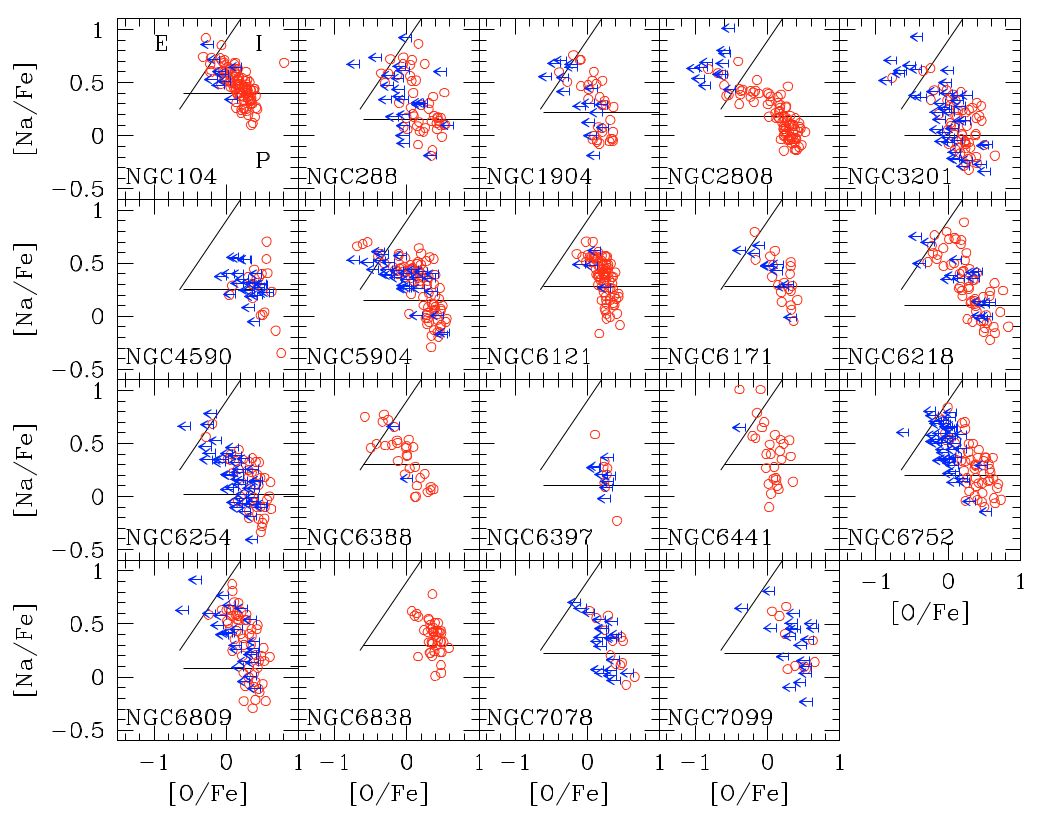
\includegraphics[width=6.5in]{Chapter-1/figs/O-Na.png}
\caption{\label{fig:O-Na}The O--Na anticorrelation of 1,200 red giants among all 19 globular clusters observed in the survey of Ref. \cite{Carretta2010}. Blue arrows indicate upper limits in O abundances, while lines separate different populations of red giants based on their relative O and Na richness. Primordial (P), extreme (E), and intermediate (I) populations are labeled in the first panel. See text for definitions of these populations. Adapted from \cite{Carretta2010}.}
\end{figure}

Fig. \ref{fig:O-Na} shows the ubiquitous O--Na anticorrelation in 1,200 red giants among all 19 globular clusters sampled by Ref. \cite{Carretta2010}. The red giants with an enhanced Na abundance are associated with a depletion in O abundance, and vice versa. The populations of red giants are split into 3 categories based on the extent of their Na enrichment, and associated O depletion. These populations are the primordial (P), extreme (E), and intermediate (I) components, as indicated in the first panel of Fig. \ref{fig:O-Na}. The primordial population is Na-poor/O-rich, the extreme population is Na-rich/O-poor, and the intermediate population is in-between. The primordial population is so-called because the same abundance pattern is typical of field stars with a similar metallicity. However, the Na and O abundances of the intermediate and extreme populations indicates that these red giants went through an unknown process. Low-mass stars like red giants and main sequence stars do not reach the high temperatures necessary for the nucleosynthesis chains that produce the observed Na and O abundances. This reasoning also applies to the other observed anticorrelations in globular clusters \cite{Prantzos2007}.

% PARAGRAPH 1: Cannot be in situ - must be mixing. Evidence for multiple stellar populations - pg 2 of Carretta2010 and Prantzos2007

% ``The (anti-)correlation among light elements is simply a manifestation of the multiple stellar populations." (Gratton et al. 2019) pg 12

% ``The variations are also found among unevolved stars currently on the main sequence (MS) of GCs (Gratton et al. 2001; Ramirez & Cohen 2002; Carretta et al. 2004; D’Orazi et al. 2010). This unequivocally implies that this composition has been imprinted in the gas by a previous generation of stars. The necessity of this conclusion stems from low-mass MS stars not being able to reach the high temperatures for the nucleosynthetic chains required to produce the observed inter-relations between the elements (in particular the Mg-Al anticorrelation). This calls for a class of now extinct stars, more massive than the low-mass ones presently evolving in GCs, as the site for the nucleosynthesis." (Carretta et al. 2010) pg 2

The most likely scenario explaining these inhomogeneities is that the currently observed stars are part of a second generation which formed from the ashes of an older, first generation of stars. The material ejected from these more-massive first generation stars upon their death likely polluted the inter-cluster medium where the second generation stars began to form. Hence, these first generation stars are sometimes called \emph{polluter stars}, a class of massive, extinct stars that are the origin of the apparent abundance anomalies. Different generations of stars exhisting in a given globular cluster would provide evidence for \emph{multiple stellar populations}. This premise has been widely debated over the last few decades, with most research supporting it at present \cite{Gratton2004,Gratton2012,Gratton2019}.

% PARAGRAPH 2: Mechanism of nucleosynthesis in second-generation globular cluster stars - H-burning. Type 1 vs type 2 globular clusters (different burning temperatures). - pg 12 of Gratton2019 - Cites Denisenkov and Denisenkova 1989; Langer et al. 1993
% Denisenkov PA, Denisenkova SN (1989) Possible explanation of the correlation between nitrogen and sodium over abundances for red giants in globular clusters. Astron Tsirkulyar 1538:11
% Langer GE, Hoffman R, Sneden C (1993) Sodium–oxygen abundance anticorrelations and deep-mixing scenarios for globular-cluster giants. Publ Astron Soc Pac 105:301–307. https://doi.org/10.1086/133147

Polluter stars are likely the site of the nucleosynthesis that gives rise to the currently observed abundance patterns in globular clusters. Their exact nature is unknown, but the nucleosynthesis mechanism driving the inhomogeneities in the vast majority of globular clusters is well established as proton-capture reactions in high temperature hydrogen-burning environments \cite{Denisenkov1989,Langer1993}. The ubiquitous O--Na anticorrelation, for example, is exhibited in the hydrogen burning of the CNO and Ne--Na cyles at about 40 MK \cite{Gratton2019}. Fig. \ref{fig:CNO_NeNa} shows the nucleosynthesis chains that lead to an overall oxygen depletion and sodium production. The first stage of the CNO cycle involves a series of $(p, \gamma)$ and $(\beta^{+}\nu)$ reactions on stable and radioactive nuclei, respectively, starting from $^{12}$C. This stage occurs at fusion temperatures of about 10 MK. Once $^{15}$N is reached, $^{15}\mathrm{N}(p, \alpha)^{12}\mathrm{C}$ closes the cycle if the temperature is less than about 40 MK. Otherwise, the second stage of the CNO cycle will be activated from $^{15}\mathrm{N}(p, \gamma)^{16}\mathrm{O}$. This eventually leads to $^{17}$O, which closes the second stage of the cycle via $^{17}\mathrm{O}(p, \alpha)^{14}\mathrm{N}$. This second stage leads to an overall destruction of oxygen. Meanwhile, the Ne--Na cycle activates at about 40 MK as well, starting from $^{20}\mathrm{Ne}(p, \gamma)^{21}\mathrm{Na}$. Once $^{23}$Na is reached, it will close the cycle via $^{23}\mathrm{Na}(p, \alpha)^{20}\mathrm{Ne}$ if temperatures are less than about 70 MK, otherwise $^{23}\mathrm{Na}(p, \gamma)^{24}\mathrm{Mg}$ is activated. These destruction reactions on $^{23}$Na are slow enough such that sodium is produced overall.

\def\BoxSpace{0.3} % Defining the variable BoxSpace to value in brackets
\def\BoxSpacetwo{\BoxSpace * 2} % So I don't have to keep doing {2+(\BoxSpace * 2)}
\def\BoxSpacethree{\BoxSpace * 3}
\def\BoxSpacehalf{\BoxSpace * 0.5}
\def\AOS{0.2} % Arrow Offset
\def\AW{0.52} % Arrow Width (mm)

\begin{figure}[t]
\centering
\noindent
\begin{minipage}{.44\linewidth}
\begin{tikzpicture}[scale=1.5, every node/.style={transform shape}]

% (0,0) is at the bottom left corner of plot, where 12C is
\filldraw[fill = light-gray] (0,0) rectangle (1,1); % 12C box
\filldraw[fill = light-gray] (1+\BoxSpace,0) rectangle (2+\BoxSpace,1); % 13C box
%\draw (2+\BoxSpacetwo,0) rectangle (3+\BoxSpacetwo,1); % 14C box
\draw (0,1+\BoxSpace) rectangle (1,2+\BoxSpace); % 13N box
\filldraw[fill = light-gray] (1+\BoxSpace,1+\BoxSpace) rectangle (2+\BoxSpace,2+\BoxSpace); % 14N box
\filldraw[fill = light-gray] (2+\BoxSpacetwo,1+\BoxSpace) rectangle (3+\BoxSpacetwo,2+\BoxSpace); % 15N box
%\draw (0,2+\BoxSpacetwo) rectangle (1,3+\BoxSpacetwo); % 14O box
\draw (1+\BoxSpace,2+\BoxSpacetwo) rectangle (2+\BoxSpace,3+\BoxSpacetwo); % 15O box
\filldraw[fill = light-gray] (2+\BoxSpacetwo,2+\BoxSpacetwo) rectangle (3+\BoxSpacetwo,3+\BoxSpacetwo); % 16O box
\filldraw[fill = light-gray] (3+\BoxSpacethree,2+\BoxSpacetwo) rectangle (4+\BoxSpacethree,3+\BoxSpacetwo); % 17O box
\draw (2+\BoxSpacetwo,3+\BoxSpacethree) rectangle (3+\BoxSpacetwo,4+\BoxSpacethree); % 17F box

\node[text=blue] at (0.5,0.5) {$^{12}\mathrm{C}$};
\node[text=red] at (1+\BoxSpace+0.5,0.5) {$^{13}\mathrm{C}$};
\node at (0.5,1+\BoxSpace+0.5) {$^{13}\mathrm{N}$};
\node[text=red] at (1+\BoxSpace+0.5,1+\BoxSpace+0.5) {$^{14}\mathrm{N}$};
\node at (2+\BoxSpacetwo+0.5,1+\BoxSpace+0.5) {$^{15}\mathrm{N}$};
\node at (1+\BoxSpace+0.5,2+\BoxSpacetwo+0.5) {$^{15}\mathrm{O}$};
\node[text=blue] at (2+\BoxSpacetwo+0.5,2+\BoxSpacetwo+0.5) {$^{16}\mathrm{O}$};
\node at (3+\BoxSpacethree+0.5,2+\BoxSpacetwo+0.5) {$^{17}\mathrm{O}$};
\node at (2+\BoxSpacetwo+0.5,3+\BoxSpacethree+0.5) {$^{17}\mathrm{F}$};

\draw[line width = \AW mm, -{Triangle[]}] (0.5,1-\AOS) -- (0.5,1+\BoxSpace+\AOS); % 12C(p,g)
\draw[line width = \AW mm, -{Triangle[]}] (1-\AOS,1+\BoxSpace+\AOS) -- (1+\BoxSpace+\AOS, 1-\AOS); % 13N(B+)
\draw[line width = \AW mm, -{Triangle[]}] (1+\BoxSpace+0.5,1-\AOS) -- (1+\BoxSpace+0.5,1+\BoxSpace+\AOS); % 13C(p,g)
\draw[line width = \AW mm, -{Triangle[]}] (1+\BoxSpace+0.5,2+\BoxSpace-\AOS) -- (1+\BoxSpace+0.5,2+\BoxSpacetwo+\AOS); % 14N(p,g)
\draw[line width = \AW mm, -{Triangle[]}] (2+\BoxSpace-\AOS,2+\BoxSpacetwo+\AOS) -- (2+\BoxSpacetwo+\AOS,2+\BoxSpace-\AOS); % 15O(B+)
\draw[line width = \AW mm, -{Triangle[]}, dashed] (2+\BoxSpacetwo+\AOS,1+\BoxSpace+\AOS) -- (1-\AOS,1-\AOS); % 15N(p,a)

\draw[line width = \AW mm, -{Triangle[]}, dashed] (2+\BoxSpacetwo+0.5,2+\BoxSpace-\AOS) -- (2+\BoxSpacetwo+0.5,2+\BoxSpacetwo+\AOS); %15N(p,g)
\draw[line width = \AW mm, -{Triangle[]}] (2+\BoxSpacetwo+0.5,3+\BoxSpacetwo-\AOS) -- (2+\BoxSpacetwo+0.5,3+\BoxSpacethree+\AOS); %16O(p,g)
\draw[line width = \AW mm, -{Triangle[]}] (3+\BoxSpacetwo-\AOS,3+\BoxSpacethree+\AOS) -- (3+\BoxSpacethree+\AOS,3+\BoxSpacetwo-\AOS); %17F(B+)
\draw[line width = \AW mm, -{Triangle[]}] (3+\BoxSpacethree+\AOS,2+\BoxSpacetwo+\AOS) -- (2+\BoxSpace-\AOS,2+\BoxSpace-\AOS); %17O(p,a)
\end{tikzpicture}
\end{minipage}
%
\begin{minipage}{.44\linewidth} \hfill
\centering
\noindent
\begin{tikzpicture}[scale=1.5, every node/.style={transform shape}]

\filldraw[fill = light-gray] (0,0) rectangle (1,1); % 20Ne box
\filldraw[fill = light-gray] (1+\BoxSpace,0) rectangle (2+\BoxSpace,1); % 21Ne box
\filldraw[fill = light-gray] (2+\BoxSpacetwo,0) rectangle (3+\BoxSpacetwo,1); % 22Ne box
\draw (0,1+\BoxSpace) rectangle (1,2+\BoxSpace); % 21Na Box
\draw (1+\BoxSpace,1+\BoxSpace) rectangle (2+\BoxSpace,2+\BoxSpace); % 22Na Box
\filldraw[fill = light-gray] (2+\BoxSpacetwo,1+\BoxSpace) rectangle (3+\BoxSpacetwo,2+\BoxSpace); % 23Na Box
\filldraw[fill = light-gray] (2+\BoxSpacetwo,2+\BoxSpacetwo) rectangle (3+\BoxSpacetwo,3+\BoxSpacetwo); %24Mg Box

\node[text=blue] at (0.5,0.5) {$^{20}\mathrm{Ne}$};
\node at (1+\BoxSpace+0.5,0.5) {$^{21}\mathrm{Ne}$};
\node at (2+\BoxSpacetwo+0.5,0.5) {$^{22}\mathrm{Ne}$};
\node at (0.5,1+\BoxSpace+0.5) {$^{21}\mathrm{Na}$};
\node at (1+\BoxSpace+0.5,1+\BoxSpace+0.5) {$^{22}\mathrm{Na}$};
\node[text=red] at (2+\BoxSpacetwo+0.5,1+\BoxSpace+0.5) {$^{23}\mathrm{Na}$};
\node at (2+\BoxSpacetwo+0.5,2+\BoxSpacetwo+0.5) {$^{24}\mathrm{Mg}$};

\draw[line width = \AW mm, -{Triangle[]}] (0.5,1-\AOS) -- (0.5,1+\BoxSpace+\AOS); %20Ne(p,g)
\draw[line width = \AW mm, -{Triangle[]}] (1-\AOS,1+\BoxSpace+\AOS) -- (1+\BoxSpace+\AOS,1-\AOS); % 21Na(B+)
\draw[line width = \AW mm, -{Triangle[]}] (1+\BoxSpace+0.5,1-\AOS) -- (1+\BoxSpace+0.5,1+\BoxSpace+\AOS); %21Ne(p,g)
\draw[line width = \AW mm, -{Triangle[]}] (2+\BoxSpace-\AOS,1+\BoxSpace+\AOS) -- (2+\BoxSpacetwo+\AOS,1-\AOS); %22Na(B+)
\draw[line width = \AW mm, -{Triangle[]}] (2+\BoxSpacetwo+0.5,1-\AOS) -- (2+\BoxSpacetwo+0.5,1+\BoxSpace+\AOS); %22Ne(p,g)
\draw[line width = \AW mm, -{Triangle[]},dashed] (2+\BoxSpacetwo+0.5,2+\BoxSpace-\AOS) -- (2+\BoxSpacetwo+0.5,2+\BoxSpacetwo+\AOS); %23Na(p,g)
\draw[line width = \AW mm, -{Triangle[]},dashed] (2+\BoxSpacetwo+\AOS,1+\BoxSpace+\AOS) -- (1-\AOS,1-\AOS); %23Na(p,a)20Ne

\end{tikzpicture}
\end{minipage}
\vspace{0.75 cm}
\caption{\label{fig:CNO_NeNa}The hydrogen burning mechanism driving the O--Na anticorrelation. Nuclei in blue are destroyed overall in the various cycles, while nuclei in red are produced. Shaded nuclei are stable. The first two stages of the CNO cycle (left), distinguished by the temperature-dependent branch at $^{15}$N, lead to an overall depletion of oxygen. The $^{15}\mathrm{N}(p, \gamma)^{16}\mathrm{O}$ reaction is activated at about 40 MK. The Ne--Na cycle (right), occurring simultaneously at about the same activation temperature, leads to an overall production of sodium. The $^{23}\mathrm{Na}(p,\gamma)^{24}\mathrm{Mg}$ reaction activates at about 70 MK.}
\end{figure}

% PARAGRAPH 3: Dilution model - mix of pristine and processed matter - pg 14 of Gratton2019

Although nucleosynthesis via hydrogen burning is what drives the observed abundance patterns, it is not the only mechanism responsible for them. The majority of second generation stars must be composed of a mixture of nuclear-processed ejecta and matter with a pristine composition, in order for nuclear reaction network models to reproduce the observed globular cluster abundance patterns \cite{Prantzos2007}. The nuclear-processed ejecta is the matter resulting from nucleosynthesis via hydrogen burning in the first generation polluter stars, while pristine matter refers to the unprocessed gas left behind from the first burst of star formation. Many polluter star sites such as AGB stars, fast-rotating massive stars, and supermassive stars require dilution with unprocessed gas in order to convert their correlated O and Na abundances into the observed anticorrelation \cite{DErcole2010,DErcole2011,DErcole2012}. The observed, mixed abundances in a typical dilution model are obtained by diluting one part of processed matter with $f$ parts of pristine matter, as in
\begin{equation} \label{eqn:mixing}
X_{\mathrm{mix}} = \frac{X_{\mathrm{proc}} + f X_{\mathrm{pris}}}{1 + f},
\end{equation}
where $X$ is the mass fraction of a given nuclide among its specific composition and $f$ is the dilution factor \cite{Prantzos2007,Carretta2009}. A very small dilution factor represents nearly pure processed matter, while a very large dilution factor results in mostly pristine matter. The dilution model works very well for most globular clusters, but often a single dilution model does not simultaneously reproduce the abundances of the extreme and intermediate populations. In these cases, more than one class of polluter stars is required to match the observations, suggesting that the multiple populations premise may be more complex than previously considered \cite{Gratton2019}.

% PARAGRAPH 4?? (Skip this): Mass-budget problem - pg 15 of Gratton2019